\documentclass[a4paper, 11pt, oneside]{article}

\usepackage[utf8]{inputenc}
\usepackage[T1]{fontenc}
\usepackage[french]{babel}
\usepackage{array}
\usepackage{shortvrb}
\usepackage{listings}
\usepackage[fleqn]{amsmath}
\usepackage{amsfonts}
\usepackage{fullpage}
\usepackage{enumerate}
\usepackage{graphicx}             % import, scale, and rotate graphics
\usepackage{subfigure}            % group figures
\usepackage{alltt}
\usepackage{url}
\usepackage{indentfirst}
\usepackage{eurosym}
\usepackage{listings}
\usepackage{color}
\usepackage[table,xcdraw,dvipsnames]{xcolor}

% Change le nom par défaut des listing
\renewcommand{\lstlistingname}{Extrait de Code}

% Change la police des titres pour convenir à votre seul lecteur
\usepackage{sectsty}
\allsectionsfont{\sffamily\mdseries\upshape}
% Idem pour la table des matière.
\usepackage[nottoc,notlof,notlot]{tocbibind}
\usepackage[titles,subfigure]{tocloft}
\renewcommand{\cftsecfont}{\rmfamily\mdseries\upshape}
\renewcommand{\cftsecpagefont}{\rmfamily\mdseries\upshape}

\definecolor{mygray}{rgb}{0.5,0.5,0.5}
\newcommand{\coms}[1]{\textcolor{MidnightBlue}{#1}}

\lstset{
    language=C, % Utilisation du langage C
    commentstyle={\color{MidnightBlue}}, % Couleur des commentaires
    frame=single, % Entoure le code d'un joli cadre
    rulecolor=\color{black}, % Couleur de la ligne qui forme le cadre
    stringstyle=\color{RawSienna}, % Couleur des chaines de caractères
    numbers=left, % Ajoute une numérotation des lignes à gauche
    numbersep=5pt, % Distance entre les numérots de lignes et le code
    numberstyle=\tiny\color{mygray}, % Couleur des numéros de lignes
    basicstyle=\tt\footnotesize,
    tabsize=3, % Largeur des tabulations par défaut
    keywordstyle=\tt\bf\footnotesize\color{Sepia}, % Style des mots-clés
    extendedchars=true,
    captionpos=b, % sets the caption-position to bottom
    texcl=true, % Commentaires sur une ligne interprétés en Latex
    showstringspaces=false, % Ne montre pas les espace dans les chaines de caractères
    escapeinside={(>}{<)}, % Permet de mettre du latex entre des <( et )>.
    inputencoding=utf8,
    literate=
  {á}{{\'a}}1 {é}{{\'e}}1 {í}{{\'i}}1 {ó}{{\'o}}1 {ú}{{\'u}}1
  {Á}{{\'A}}1 {É}{{\'E}}1 {Í}{{\'I}}1 {Ó}{{\'O}}1 {Ú}{{\'U}}1
  {à}{{\`a}}1 {è}{{\`e}}1 {ì}{{\`i}}1 {ò}{{\`o}}1 {ù}{{\`u}}1
  {À}{{\`A}}1 {È}{{\`E}}1 {Ì}{{\`I}}1 {Ò}{{\`O}}1 {Ù}{{\`U}}1
  {ä}{{\"a}}1 {ë}{{\"e}}1 {ï}{{\"i}}1 {ö}{{\"o}}1 {ü}{{\"u}}1
  {Ä}{{\"A}}1 {Ë}{{\"E}}1 {Ï}{{\"I}}1 {Ö}{{\"O}}1 {Ü}{{\"U}}1
  {â}{{\^a}}1 {ê}{{\^e}}1 {î}{{\^i}}1 {ô}{{\^o}}1 {û}{{\^u}}1
  {Â}{{\^A}}1 {Ê}{{\^E}}1 {Î}{{\^I}}1 {Ô}{{\^O}}1 {Û}{{\^U}}1
  {œ}{{\oe}}1 {Œ}{{\OE}}1 {æ}{{\ae}}1 {Æ}{{\AE}}1 {ß}{{\ss}}1
  {ű}{{\H{u}}}1 {Ű}{{\H{U}}}1 {ő}{{\H{o}}}1 {Ő}{{\H{O}}}1
  {ç}{{\c c}}1 {Ç}{{\c C}}1 {ø}{{\o}}1 {å}{{\r a}}1 {Å}{{\r A}}1
  {€}{{\euro}}1 {£}{{\pounds}}1 {«}{{\guillemotleft}}1
  {»}{{\guillemotright}}1 {ñ}{{\~n}}1 {Ñ}{{\~N}}1 {¿}{{?`}}1
}
\newcommand{\tablemat}{~}

%%%%%%%%%%%%%%%%% TITRE %%%%%%%%%%%%%%%%
% Complétez et décommentez les définitions de macros suivantes :
\newcommand{\intitule}{Projet1}
\newcommand{\GrNbr}{06}
\newcommand{\PrenomUN}{Maxime}
\newcommand{\NomUN}{Deravet}
\newcommand{\PrenomDEUX}{Luca}
\newcommand{\NomDEUX}{Matagne}
% Décommentez ceci si vous voulez une table des matières :
\renewcommand{\tablemat}{\tableofcontents}

%%%%%%%% ZONE PROTÉGÉE : MODIFIEZ UNE DES DIX PROCHAINES %%%%%%%%
%%%%%%%%            LIGNES POUR PERDRE 2 PTS.            %%%%%%%%
\title{INFO0947: \intitule}
\author{Groupe \GrNbr : \PrenomUN~\textsc{\NomUN}, \PrenomDEUX~\textsc{\NomDEUX}}
\date{}
\begin{document}

\maketitle
\newpage
\tablemat
\newpage
%%%%%%%%%%%%%%%%%%%% FIN DE LA ZONE PROTÉGÉE %%%%%%%%%%%%%%%%%%%%

%%%%%%%%%%%%%%%% RAPPORT %%%%%%%%%%%%%%%
% Écrivez votre rapport ci-dessous.

\section{Formalisation du problème}
\subsection{Objets utilisés}

T est un tableau d'entiers de taille non nulle
\\
N est la taille du tableau T,  (N \textgreater 0)
\\
taille\_utile est le nombre d'éléments du tableau qui satisfont $p(.) (0 \leq taille\_utile \leq N  )$

\subsection{Prédicats}
p(x) est un prédicat déjà défini 
\\
\\
$Zone\_utile(T_{0},  N)  \equiv \#j \cdot (0\leq j < N|  p(T_{0}[j]))  $
\\
\\
$Filtrage(T_{0}, N,taille\_utile)\equiv \forall j, 0 \leq j < taille\_utile, p(T_{0}[j])$\\
\\
$Zone\_morte(T, N,taille\_utile)\equiv \forall j, taille\_utile \leq j < N, T[j] = 0$ 
\\
\\
$Sous\_suite(T_0, taille\_utile, T, N)\equiv (\forall k, 1 \leq k < taille\_utile, (\exists j, 0 \leq j<N, T_0[j]=T[k]))\land(\exists l, o \leq l < j, T_0[l]=T[k-1]) $


\section{Spécifications du module}


\begin{lstlisting}
/**
 *
 * @préconditions : (>\coms{ $ \forall T[i], 0 \leq i < N, T[i] \in \mathbb{Z}
                    \land
                    N > 0$  }<)
 * @postconditions : (>\coms{ $ N=N_0
                     \land 
                     filtrer(T, N) = taille\_utile
                     \land 
                     T = [(Sous\_suite(T_0, taille\_utile, T, N) \land Filtrage(T_0, N, taille\_utile) || Zone\_morte(T,N,taille\_utile))] $  }<)
 */
int filtrer(int *T, int N);

\end{lstlisting}



\section{Découpe en sous-problèmes}
SP0 : Parcours du tableau et vérification de  $p(\cdot)$ pour chaque valeur
\\SP1 : Si p n'est pas vérifié, on place un 0 dans la case actuelle, et on continue le parcours du tableau
\\SP2 : Si p est vérifié, on vérifie si on a déjà rencontré des valeurs qui ne vérifient pas p
\\SP2.1 : si c'est le cas, alors on met la valeur actuelle dans la case à l'index taille\_utile, puis 0 dans la case actuelle. On incrément taille\_utile. On poursuis la boucle ensuite
\\SP2.2. Si on n'a pas encore rencontré de valeur ne vérifiant pas p, alors on incrémente taille\_utile, et on poursuis la boucle. 

$SP0 \supset (SP1, SP2 \supset (SP2.1, SP2.2))$



\section{Invariants de boucle}
Le SP0 fait apparaître la nécessité d'une boucle pour résoudre le problème. 
Voici les invariants de cette boucle:

\subsection{Invariant graphique}
\begin{wrapfigure}{Invariant graphique de la fonction filtrer()}

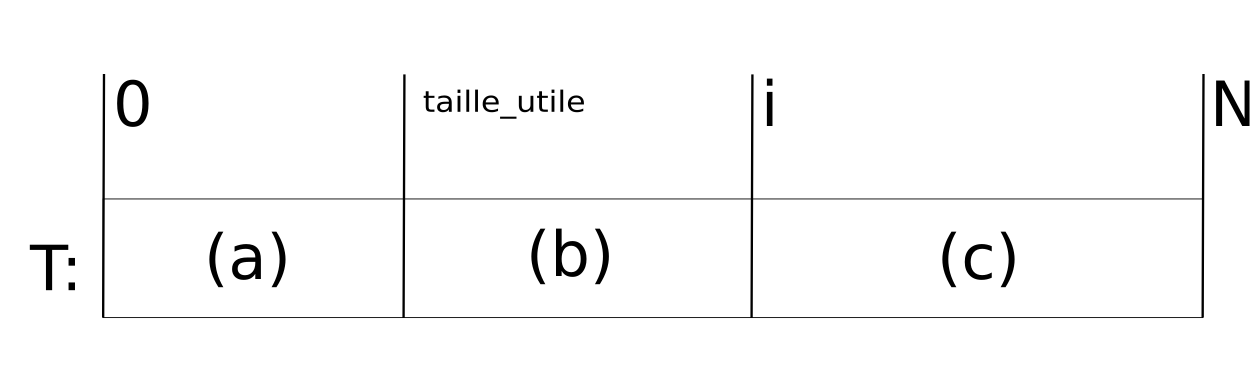
\includegraphics[scale = 0.5]{Capture d’écran 2022-03-23 165331.png}
\end{wrapfigure}

a) Les valeurs vérifient $p(\cdot)$ et sont dans le même ordre que $T_{0}$\\
b) Contient des 0 (il y en a i - taille\_utile)\\
c) Le tableau n'est pas encore filtré\\



\subsection{Invariant formel}
$N = N_{0} 
\\ \land 0 \leq taille\_utile \leq i < N
\\ \land \forall x, 0 \leq x<taille\_utile, Filtrage(T_{0}, i, taille\_utile), Sous\_suite(T_0, taille\_utile, T, i) 
\\ \land \forall y, taille\_utile \leq y<i, Zone\_morte(T, i, taille\_utile) $
\\
\\
fonction de terminaison : N-i
\section{Implémentations des Sous-Problèmes}
\subsection{SP0}
\begin{lstlisting}
while(i<N){ //SP0
        if(!test(T[i])){ //SP0
        //SP1
        }else{
        //SP2
        }
    }
\end{lstlisting}
\subsection{SP1}
\begin{lstlisting}
if(!test(T[i])){//SP0
   T[i]= 0;//SP1
   i++;//SP1
   }
\end{lstlisting}

\subsection{SP2}
\begin{lstlisting}
else{//SP0
    if(taille_utile!= i){//SP2
        T[taille_utile]= T[i];//SP2.1
        T[i]= 0;//SP2.1
        i++;//SP2.1
        taille_utile++;//SP2.1
    }else{//SP2
        taille_utile++;//SP2.2
        i++;//SP2.2
    }
\end{lstlisting}


\section{Construction du code}

\subsection{Code complet}
\begin{lstlisting}
int filtrer(int *T, int N){
    assert(T != NULL && N >0);
    // $\forall T[i], 0 \leq i < N, T[i] \in \mathbb{Z} \land N < 0 $
    int i= 0;
    int taille_utile = 0;
    // $\forall T[i], 0 \leq i < N, T[i] \in \mathbb{Z} \land N < 0 \land i = 0 \land taille\_utile = 0 $ 

    // $ N = N_{0} $
    // $ \land $
    // $0 \leq taille\_utile \leq i < N $
    // $ \land $
    // $ \forall x, 0 \leq x < taille\_utile, Filtrage(T_{0}, N, taille\_utile),  Sous\_Suite(T_{0}, taille\_utile, T, N) $
    // $ \land $
    // $ \forall y, taille\_utile \leq y<i, Zone\_morte(T, i, taille\_utile) $
    while(i<N){
    // $ N = N_{0} $
    // $ \land $
    // $ 0 \leq taille\_utile \leq i < N $
    // $ \land $
    // $ \forall x, 0 \leq x < taille\_utile, Filtrage(T_{0}, i, taille\_utile),  Sous\_Suite(T_{0}, taille\_utile, T, i) $
    // $ \land $
    // $ \forall y, taille\_utile \leq y<i, Zone\_morte(T, i, taille\_utile) $
    // $ \land $
    // $ i < N $
        if(!test(T[i])){
        // $ Filtrage(T_{0}, i-1, taille\_utile-1) \land  Zone\_Morte(T, i-1, taille\_utile-1) \land \neg p(T[i]) $
            T[i]= 0;
            // $ Filtrage(T_{0}, i, taille\_utile-1) \land  Zone\_Morte(T, i, taille\_utile-1) $
            i++;
            // $ Filtrage(T_{0}, i-1, taille\_utile-1) \land  Zone\_Morte(T, i-1, taille\_utile-1) $
        }else{
        // $ Filtrage(T_{0}, i-1, taille\_utile-1) \land  Zone\_Morte(T, i-1, taille\_utile-1) \land p(T[i]) $
            if(taille_utile!= i){
            // $ Filtrage(T_{0}, i-1, taille\_utile-1) \land  Zone\_Morte(T, i-1, taille\_utile-1)$
            // $ \land $
            // $ p(T[i]) \land taille\_utile \neq i $
                T[taille_utile]= T[i];
                T[i]= 0;
                // $ Filtrage(T_{0}, i, taille\_utile) \land  Zone\_Morte(T, i, taille\_utile) $
                // $ \land $
                // $ taille\_utile \neq i $
                i++;
                taille_utile++;
                // $ Filtrage(T_{0}, i-1, taille\_utile-1) \land  Zone\_Morte(T, i-1, taille\_utile-1) $
                // $ \land $
                // $ taille\_utile \neq i $
            }else{
            // $ Filtrage(T_{0}, i-1, taille\_utile-1) \land  Zone\_Morte(T, i-1, taille\_utile-1)$
            // $ \land $
            // $ p(T[i]) \land taille\_utile = i $
                taille_utile++;
                i++;
                //HHHHHHHHHHHEEEEEEEEEEEERRRRRRRRRREEEEEEEEEE
            }
        }
    }//fin while
    // $ N = N_{0} $
    // $ \land $
    // $ 0 \leq taille\_utile \leq i < N $
    // $ \land $
    // $ \forall x, 0 \leq x < taille\_utile, Filtrage(T_{0}, i, taille\_utile),  Sous\_Suite(T_{0}, taille\_utile, T, i) $
    // $ \land $
    // $ \forall y, taille\_utile \leq y<i, Zone\_morte(T, i, taille\_utile) $
    // $ \land $
    // $ i \geq N $
    return taille_utile;
    // $ N = N_{0} $
    // $ \land $
    // $ filtrer(T, N) = taille\_utile $
    // $ \land $
    // $ T = [(Sous\_suite(T_0, taille\_utile, T, N) \land Filtrage(T_0, N, taille\_utile))|| Zone\_morte(T,N,taille\_utile)] $
}//fin filtrer
\end{lstlisting}

\section{Démonstration de la complexité de $filtrer()$}
Construisons la fonction T($\cdot$), qui est la somme des complexités de chaque partie de $filtrer()$:


La première partie du code regroupe les initialisations de variables et est appelée T(A). La boucle $while$ et son contenu seront regroupés dans la fonction T(B). Et pour terminer, l'instruction $return$ sera reprise dans la fonction T(C).

\subsection{T(A)}

\begin{lstlisting}
    assert(T != NULL && N >0);
    int i= 0;
    int taille_utile = 0;
\end{lstlisting}

T(A) regroupe uniquement des déclarations et vérifications de variables. Selon la règle 1 (cfr. INFO0946, chapitre 4),nous pouvons dire que T(A) = 1.


\subsection{T(B)}

\begin{lstlisting}
while(i<N){
          
        if(!test(T[i])){
            T[i]= 0;
            i++;
            
        }else{
            if(taille_utile!= i){
                T[taille_utile]= T[i];
                T[i]= 0;
                i++;
                taille_utile++;
            }else{
                taille_utile++;
                i++;
            }
        }
    }//fin while
\end{lstlisting}
Selon la règle 5, la complexité d'une boucle $while$, est la complexité du contenu multipliée par le nombre de tours.

Intéressons-nous donc au contenu: 
Pour commencer, nous avons une première structure $if$ $else$. Sous le premier $if$ se trouvent uniquement des affectations et incrémentations de variables. Selon la règle 2, la complexité théorique est donc $T_1(n)$. 


Ensuite, sous le premier $else$, se trouve une deuxième structure $if$ $else$. Regardons ce qu'il s'y trouve:

Encore une fois, sous le second $if$, se trouvent uniquement des opérations d'incrémentations et d'affectations de variables. La complexité théorique est $T\_3(n)$(selon la règle 2). 

Sous le second $else$, de nouveau, seulement des incrémentations de variables, et donc une complexité théorique $T_4(n)$ (selon la règle 2). 


En additionnant le tout, cela nous donne : 
$T_2(n) =  max(T_3(n), T_4(n))$
\\i est le nombre de tours de boucle
\begin{align}
  T(B) &= max(T_1(n), T_2(n)) * i\nonumber \\
       &= T(n) * i  \nonumber \\
       &=T(n) \nonumber
\end{align}

Voici un schéma reprenant les explications ci-dessus:
\\
\begin{wrapfigure}
\centering \includegraphics[scale = 0.8]{Complexité.png}
\end{wrapfigure}

\subsection{T(C)}

Étant donné que la fonction T(C) ne reprend qu'une seule instruction, qui est le $return$, sa complexité est égale à 1 (règle 1).

\subsection{Complexité du module complet}

Au final, nous obtenons :

\begin{align}
  T(N) &= T(A) + T(B) + T(C) \nonumber \\
       &= 1 + n + 1 \nonumber \\
       &= n + 2 \nonumber \\
       &= n
\end{align}
La complexité du module $filtrer$ est donc \bf linéaire.
\end{document}
